\documentclass[tikz]{standalone}
\usepackage{tikz,amsmath}
\usetikzlibrary{calc}
\tikzstyle{vertex} = [draw, shape=circle, minimum width=.3cm, inner sep=.5pt]
% Shared palette and panel style for the book's tikz diagrams.
%
% The colours are derived from the illustrations of James Brown
% (nonzerosum.games), so that the diagrams and the illustrations read as one
% visual family. Every illustration sits on a grey canvas, is outlined in heavy
% near-black ink, and draws its fills from a small set of muted hues.
%
% The three data colours (gtbblue, gtbterracotta, gtbyellow) were chosen to
% remain distinguishable from each other, and from the canvas, under simulated
% deuteranomaly, protanomaly and tritanomaly. Their worst-case CAM02-UCS
% separation is 34.5, against 11.7 for the Okabe-Ito palette they replace.
% Do not adjust these values without rerunning tests/test_palette.py, which
% guards that property.
%
% Usage: \input this file in a standalone diagram preamble. The grey panel is
% applied to every tikzpicture automatically; no per-picture option is needed.

\usepackage{xcolor}
\usepackage{tikz}
\usetikzlibrary{backgrounds}

% Structural colours.
\definecolor{gtbink}{HTML}{2B2A29}    % outlines and text
\definecolor{gtbcanvas}{HTML}{C3C3C3} % panel background
\definecolor{gtbpaper}{HTML}{FAFAFA}  % node fills, echoing the speech bubbles

% Data colours, verified colourblind-safe on the canvas.
\definecolor{gtbblue}{HTML}{5B90C6}
\definecolor{gtbterracotta}{HTML}{935B39}
\definecolor{gtbyellow}{HTML}{EBBF33}

% Supporting colours from the same illustrations, for diagrams needing more
% than three. These are not part of the verified trio.
\definecolor{gtbcoral}{HTML}{D1723B}
\definecolor{gtbviolet}{HTML}{5D57A1}
\definecolor{gtbsage}{HTML}{74A8AF}
\definecolor{gtbmuted}{HTML}{555555}

\tikzset{
  gtb panel/.style={
    background rectangle/.style={fill=gtbcanvas, rounded corners=8pt},
    show background rectangle,
    inner frame sep=14pt,
  },
  % `color` sets the default for strokes, fills and text at once, so unadorned
  % \draw and \node pick up the ink colour. Explicit fill=/draw= still win.
  every picture/.append style={gtb panel, color=gtbink},
}

\begin{document}
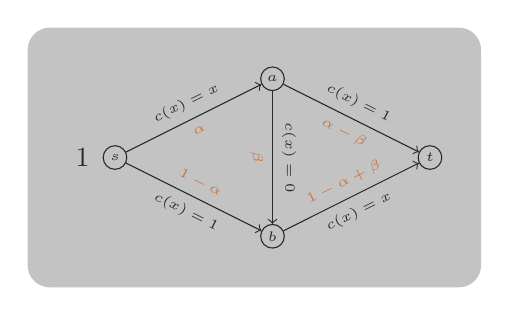
\begin{tikzpicture}[sloped]
    \draw (-1,0) node[vertex] (s) {\tiny{$s$}};
    \draw (1,1) node[vertex] (a) {\tiny{$a$}};
    \draw (1,-1) node[vertex] (b) {\tiny{$b$}};
    \draw (3,0) node[vertex] (t) {\tiny{$t$}};
    \draw [->] (s) -- node [above] {\tiny{$c(x)=x$}} node [below,gtbcoral] {\tiny{$\alpha$}} (a);
    \draw [->] (s) -- node [below] {\tiny{$c(x)=1$}} node [above,gtbcoral] {\tiny{$1-\alpha$}} (b);
    \draw [->] (a) -- node [above] {\tiny{$c(x)=1$}} node [below,gtbcoral] {\tiny{$\alpha-\beta$}} (t);
    \draw [->] (b) -- node [below] {\tiny{$c(x)=x$}} node [above,gtbcoral] {\tiny{$1-\alpha+\beta$}} (t);
    \draw [->] (a) -- node [above]{\tiny{$c(x)=0$}} node [below,gtbcoral] {\tiny{$\beta$}} (b);
    \node at (s) [left=.2cm] {$\tiny{1}$};
\end{tikzpicture}
\end{document}
